% -*- coding: utf-8 -*-
% !TEX program = xelatex

\documentclass[9pt]{beamer}

\usetheme[style=beta]{epyt} % alpha, beta, delta, gamma, zeta
%\usetheme{Warsaw}
\usepackage[UTF8,noindent]{ctex}
%%%% \renewcommand *****
%\renewcommand{\lstlistingname}{}
%\newcommand{\tf}{\ttfamily}
%\newcommand{\ttt}{\texttt}
%\newcommand{\blue}{\textcolor{blue}}
%\newcommand{\red}{\textcolor{red}}
%\newcommand{\purple}{\textcolor{purple}}
\newcommand{\ft}{\frametitle}
\newcommand{\fst}{\framesubtitle}
\newcommand{\bs}{\boldsymbol}
\newcommand{\ds}{\displaystyle}
\newcommand{\vd}{\vdots}
\newcommand{\cd}{\cdots}
\newcommand{\dd}{\ddots}
\newcommand{\id}{\iddots}
\newcommand{\XX}{\mathbf{X}}
\newcommand{\PP}{\mathbf{P}}
\newcommand{\QQ}{\mathbf{Q}}
\newcommand{\xx}{\mathbf{x}}
\newcommand{\yy}{\mathbf{y}}
\newcommand{\bb}{\mathbf{b}}
\newcommand{\abd}{\boldsymbol{a}}
%\newcommand{\A}{\mathbf{A}}
%\newcommand{\B}{\mathbf{B}}
%\newcommand{\C}{\mathbf{C}}
%\newcommand{\D}{\mathbf{D}}
%\newcommand{\E}{\mathbf{E}}
%\newcommand{\X}{\mathbf{X}}
%\newcommand{\Y}{\mathbf{Y}}
%\newcommand{\Z}{\mathbf{Z}}
\newcommand{\R}{\mathbb{R}}
%\newcommand{\T}{\mathbf{T}}
%\newcommand{\zero}{\mathbf{0}}
%\newcommand{\II}{\mathbf{I}}
%\newcommand{\LLambda}{\mathbf{\Lambda}}
%\newcommand{\alphabd}{\boldsymbol{\alpha}}
%\newcommand{\betabd}{\boldsymbol{\beta}}
%\newcommand{\gammabd}{\boldsymbol{\gamma}}
%
%\newcommand{\Loc}{\mathrm{Loc}}

%\input{macro/newtheorem}
%% \usepackage[T1]{fontenc} % Needed for Type1 Concrete
%% %% \usepackage{concrete} % Loads Concrete + Euler VM
%% %% \usepackage{pxfonts} % Or palatino or mathpazo
%% \usepackage{eulervm} %
%% %% \usepackage{kerkis} % Kerkis roman and sans
%% %% \usepackage{kmath} % Kerkis math
%% \usepackage{fourier}
\usepackage{etex}
\usepackage{pgf}
\usepackage{tikz}
\usetikzlibrary{calc}
\usetikzlibrary{arrows,snakes,backgrounds,shapes,shadows}
\usetikzlibrary{matrix,fit,positioning,decorations.pathmorphing}
\usepackage{CJK} 
\usepackage{amsmath,amssymb,amsfonts}
\usepackage{mathdots}
\usepackage{caption}
\usepackage{verbatim,color,xcolor}
\usepackage{graphicx}
\usepackage{manfnt}
\usepackage{fancybox}
\usepackage{textcomp}
\usepackage{multirow,multicol}
\usepackage{parcolumns}
\usepackage{framed}
\usepackage{threeparttable}
\usepackage{extarrows}
\usepackage{listings}
\lstset{
  keywordstyle=\color{blue!70},
  frame=single,
  basicstyle=\ttfamily\small,
  commentstyle=\small\color{red},
  breakindent=0pt,
  rulesepcolor=\color{red!20!green!20!blue!20},
  rulecolor=\color{black},
  tabsize=4,
  numbersep=5pt,
  breaklines=true,
  %% backgroundcolor=\color{red!10},
  showspaces=false,
  showtabs=false,
  extendedchars=false,
  escapeinside=``,
  frame=no,
}
%% \usepackage[utf8]{inputenc}
%% \usepackage[upright]{fourier}   %


%\usepackage{xcolor}
%\usepackage{pgf}
%\usepackage{tikz}
\usepackage{pgfplots}
%\usetikzlibrary{calc}
%\usetikzlibrary{arrows,snakes,backgrounds,shapes}
%\usetikzlibrary{matrix,fit,positioning,decorations.pathmorphing}
%\usepackage{CJK}               
%\usepackage[italian,american]{babel}
%\usepackage[applemac]{inputenc}
%\usepackage[T1]{fontenc}
%\usepackage{amsmath,amssymb,amsthm}
%\usepackage{varioref}
%\usepackage[style=philosophy-modern,hyperref,square,natbib]{biblatex}
%\usepackage{chngpage}
%\usepackage{calc}
%\usepackage{listings}
%\usepackage{graphicx}
\usepackage{subfigure}
%\usepackage{multicol}
%\usepackage{makeidx}
%\usepackage{fixltx2e}
%\usepackage{relsize}
%\usepackage{lipsum}
\usepackage{xifthen}
%%% \usepackage[eulerchapternumbers,subfig,beramono,eulermath,pdfspacing,listings]{classicthesis}
%%% \usepackage{arsclassica}        
%\usepackage{titlesec} %设置标题
%\usepackage{titletoc}
%\usepackage{extarrows}
%\usepackage{enumerate}

\input{macro/newenviroment}

\newcommand{\mylead}[1]{\textcolor{acolor1}{#1}}
\newcommand{\mybold}[1]{\textcolor{acolor2}{#1}}
\newcommand{\mywarn}[1]{\textcolor{acolor3}{#1}}



\begin{document}

\title{数据结构与算法}
\subtitle{基本数据结构}
\author{张晓平}
\institute{武汉大学数学与统计学院}


\begin{frame}[plain]\transboxout
\titlepage
\end{frame}

\section*{目录}
\frame{  
        \frametitle{\secname}
        \begin{multicols}{2}  %两行目录
                \tableofcontents
        \end{multicols}
}
\AtBeginSection[] {  %在每个subsection前面显示一次目录
        \frame{
                \frametitle{\secname}
                \begin{multicols}{2}  %两行目录
                        \tableofcontents[current,currentsection]
                \end{multicols}
        }
}

\AtBeginSubsection[] {  %在每个subsection前面显示一次目录
        \frame{
                \frametitle{\secname}
                \begin{multicols}{2}  %两行目录
                        \tableofcontents[current,currentsubsection]
                \end{multicols}
        }
}


\section{目标}
\begin{frame}[fragile]\ft{\secname}

\begin{itemize}
        \item 理解抽象数据类型的栈,队列,deque 和列表。
        \item 能使用 Python 列表实现 ADT 堆栈,队列和 deque。
        \item 了解基本线性数据结构实现的性能。
        \item 了解前缀、中缀和后缀表达式格式。
        \item 使用栈来实现后缀表达式。
        \item 使用栈将中缀表达式转换为后缀表达式。
        \item 使用队列进行基本时序仿真。
        \item 学会在问题中合理的使用栈、队列和 deques 等数据结构。
        \item 能使用节点和引用将列表实现转换为链表实现。
        \item 能比较链表实现与 Python 的列表实现的性能。
\end{itemize}
\end{frame}

\section{线性数据结构}
\begin{frame}\ft{\secname} 
我们从四个简单但重要的概念开始研究数据结构:
\begin{enumerate}
        \item 栈(stack)
        \item 队列(sequence)
        \item 双端列表(deque)
        \item 列表(list)
\end{enumerate}
它们都是一类数据的容器,数据项之间的顺序由添加或删除的顺序决定。一旦一个数据项被添加,它相对于前后元素一直保持该位置不变。
诸如此类的数据结构被称为线性数据结构。
\end{frame}


\begin{frame}\ft{\secname} 
线性数据结构有两端,有时被称为左、右,某些情况被称为前、后。你也可以称为顶部和底部,名字都不重要。 将两个线性数据结构区分开的方法是添加和移除项的方式,特别是添加和移除项的位置。  例如一些结构允许从一端添加项,另一些允许从另一端移除项。这些变种的形式产生了计算机科学最有用的数据结构。他们出现在各种算法中,并可以用于解决很多重要的问题。
\end{frame}
 
\section{栈}
\begin{frame}\ft{\secname}
栈是一个项的有序集合,其中添加移除新项总发生在同一端。这一端通常称为“顶部”,与顶部对应的端称为“底部”。
\begin{itemize}
        \item 栈的底部很重要,因为在栈中靠近底部的项是存储时间最长的。
        \item 最近添加的项是最先会被移除的。这种排序原则有时被称为 LIFO(last in first out),后进先出。
        \item 它基于在集合内的时间长度做排序。较新的项靠近顶部,较旧的项靠近底部。
\end{itemize}
\end{frame}
%
\subsection{栈的举例}
\begin{frame}\ft{\subsecname}

\begin{testexample} 
几乎所有的自助餐厅都有一堆托盘或盘子,你从顶部拿一个,就会有一个新的托盘给下一个客人。  
\end{testexample}
\end{frame}

\begin{frame}\ft{\subsecname}
\begin{testexample} 
想象桌上有一堆书, 只有顶部的那本书封面可见,要看到其他书的封面,只有先移除他们上面的书。

\centering
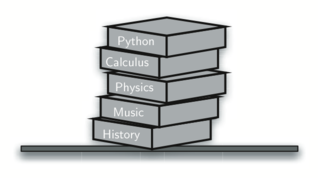
\includegraphics[width=3in]{images/WhatIsStack1.png}
\end{testexample}
        
        
\end{frame}

\begin{frame}\ft{\subsecname}
\begin{testexample} 
下图展示了另一个栈,包含了很多 Python 对象。

\centering
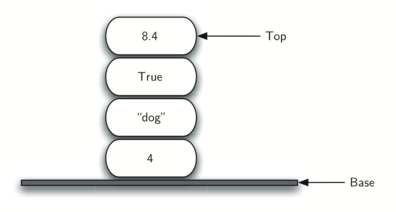
\includegraphics[width=3in]{images/WhatIsStack2.png}
\end{testexample}       
\end{frame}

\begin{frame}\ft{\subsecname}
\begin{testexample} 
和栈相关的最有用的想法之一来自对它的观察。
假设从一个干净的桌面开始,现在把书一本本叠起来,你在构造一个栈。考虑下移除一本书会发生什么。移除的顺序跟刚刚被放置的顺序相反。栈之所以重要是因为它能反转项的顺序。插入跟删除顺序相反,下图展示了 Python 数据对象创建和删除的过程,注意观察他们的顺序。

\centering
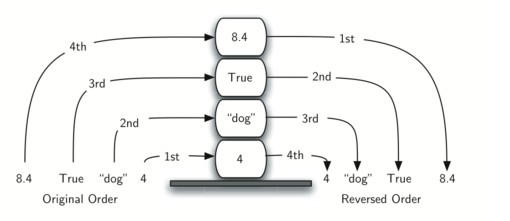
\includegraphics[width=4in]{images/WhatIsStack3.png}
\end{testexample}
\end{frame}

\begin{frame}\ft{\subsecname}
\begin{testexample} 
想想这种反转的属性,你可以想到使用计算机的时候所碰到的例子。例如,每个 web 浏览器都有一个返回按钮。当你浏览网页时,这些网页被放置在一个栈中(实际是网页的网址)。你现在查看的网页在顶部,你第一个查看的网页在底部。如果按‘返回’按钮,将按相反的顺序浏览刚才的页面。
\end{testexample}

\end{frame}


\subsection{栈的抽象数据类型}
\begin{frame}\ft{\subsecname}
栈的抽象数据类型由以下结构和操作定义。如上所述,栈被构造为项的有序集合,其中项被添加和从末端移除的位置称为“顶部”。栈是有序的 LIFO 。栈操作如下:
\begin{enumerate}
        \item { Stack()}: 创建一个空的新栈。 它不需要参数,并返回一个空栈。
        \item { push(item)}: 将一个新项添加到栈的顶部。它需要 item 做参数并不返回任何内容。
        \item { pop()}: 从栈中删除顶部项。它不需要参数并返回 item 。栈被修改。
        \item { peek()}: 从栈返回顶部项,但不会删除它。不需要参数。 不修改栈。
        \item { isEmpty()}: 测试栈是否为空。不需要参数,并返回布尔值。
        \item { size()}: 返回栈中的 item 数量。不需要参数,并返回一个整数。 
\end{enumerate}
\end{frame}
 
\begin{frame}\ft{\subsecname}
\begin{figure}[htbp]
        \centering
        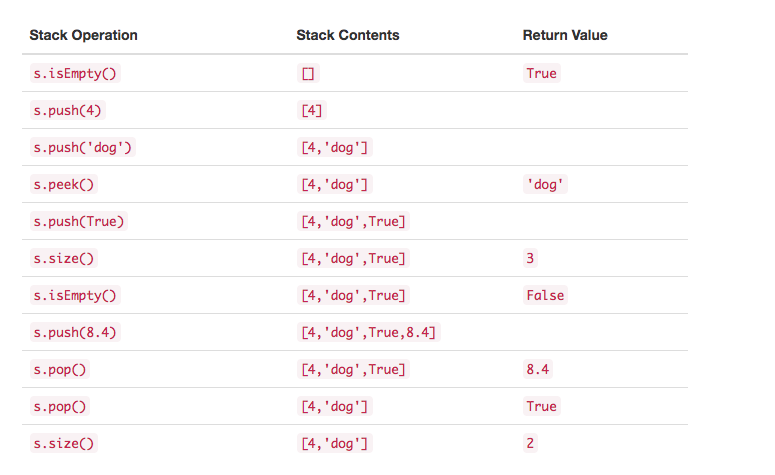
\includegraphics[width=5in]{images/stack_table1.png}
\end{figure}
\end{frame}


\subsection{用 Python 实现栈}

\begin{frame}\ft{\subsecname}
现在我们已经将栈清楚地定义了抽象数据类型,我们将把注意力转向使用 Python 实现栈。回想一下,当我们给抽象数据类型一个物理实现时,我们将实现称为数据结构。
正如我们在第1章中所描述的,在 Python 中,与任何面向对象编程语言一样,抽象数据类型(如栈)的选择的实现是创建一个新类。栈操作实现为类的方法。此外,为了实现作为元素集合的栈,使用由 Python 提供的原语集合的能力是有意义的。 我们将使用列表作为底层实现。
\end{frame}


\begin{frame}\ft{\subsecname}
回想一下,Python 中的列表类提供了有序集合机制和一组方法。例如,如果我们有列表 {\tf [2, 5, 3, 6, 7, 4]},我们只需要确定列表的哪一端将被认为是栈的顶部。一旦确定,可以使用诸如 {\tf append} 和 {\tf pop} 的列表方法来实现操作。
以下栈实现假定列表的结尾将保存栈的顶部元素。随着栈增长({\tf push} 操作),新项将被添加到列表的末尾。 {\tf pop} 也操作列表末尾的元素。
\end{frame}


\begin{frame}[fragile]\ft{\subsecname}
\lstinputlisting{code/stack_class.py}
注意这里只定义了类的实现,我们需要创建一个栈,然后使用它。
\end{frame}


\begin{frame}[fragile]\ft{\subsecname}
以下代码展示了我们通过实例化 Stack 类执行上述表格中的操作。注意,Stack 类的定义是从 pythonds 模块导入的。

\begin{lstlisting}[language=python,frame=single]
s=Stack()

print(s.isEmpty())
s.push(4)
s.push('dog')
print(s.peek())
s.push(True)
print(s.size())
print(s.isEmpty())
s.push(8.4)
print(s.pop())
print(s.pop())
print(s.size())
\end{lstlisting}
\end{frame}
%
\subsection{栈的应用}


\subsubsection{简单括号匹配}
\begin{frame}[fragile]\ft{\subsubsecname}
我们现在把注意力转向使用栈解决真正的计算机问题。

\begin{itemize}
\item 你会这么写算术表达式
\begin{lstlisting}
(5 + 6) * (7 + 8) / (4 + 3)
\end{lstlisting}
其中括号用于命令操作的执行。
\item 
你可能也有一些语言的经验,如 Lisp 的构造
\begin{lstlisting}
(defun square(n) (* n n))
\end{lstlisting}
这段代码定义了一个名为 square 的函数,它将返回参数的 n 的平方。 Lisp 使用大量的圆括号是臭名昭著的。
\end{itemize}
\end{frame}

\begin{frame}[fragile]\ft{\subsubsecname}
在这两个例子中,括号必须以匹配的方式出现。括号匹配意味着每个开始符号具有相应的结束符号,并且括号能被正确嵌套。考虑下面正确匹配的括号字符串:
\begin{lstlisting}
( ( ) ( ) ( ) ( ) )
( ( ( ( ) ) ) )
( ( ) ( ( ( ) ) ( ) ) )
\end{lstlisting}
对比那些不匹配的括号:
\begin{lstlisting}
( ( ( ( ( ( ( ) )
( ) ) )
( ( ) ( ) ( ( )
\end{lstlisting}
\end{frame}

\begin{frame}[fragile]\ft{\subsubsecname}
区分括号是否匹配的能力是识别很多编程语言结构的重要部分。具有挑战的是如何编写一个算法,能够从左到右读取一串符号,并决定符号是否平衡。为了解决这个问题,我们需要做一个重要的观察: 从左到右处理符号时,最近开始符号必须与下一个关闭符号相匹配
此外,处理的第一个开始符号必须等待直到其匹配最后一个符号。
结束符号以相反的顺序匹配开始符号。
他们从内到外匹配。
这是一个可以用栈解决问题的线索。
\begin{figure}[htbp]
        \centering
        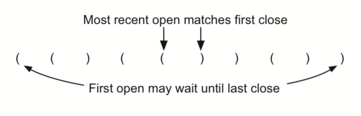
\includegraphics[width=4in]{images/simpleparcheck.png}
\end{figure}
\end{frame}

\begin{frame}[fragile]\ft{\subsubsecname}
一旦你认为栈是保存括号的恰当的数据结构,算法是很直接的。从空栈开始,从左到右处理括号字符串。如果一个符号是一个开始符号,将其作为一个信号,对应的结束符号稍后会出现。另一方面,如果符号是结束符号,弹出栈,只要弹出栈的开始符号可以匹配每个结束符号,则括号保持匹配状态。如果任何时候栈上没有出现符合开始符号的结束符号,则字符串不匹配。最后,当所有符号都被处理后,栈应该是空的。
\end{frame}

\begin{frame}[fragile]\ft{\subsubsecname}
\lstinputlisting{code/parsecheck.py}
\end{frame}

\begin{frame}[fragile]\ft{\subsubsecname}
\begin{lstlisting}
print(parChecker('((()))'))
print(parChecker('(()'))
\end{lstlisting}
\begin{lstlisting}[frame=no]
True
False
\end{lstlisting} 
\end{frame}
\end{document}
